\documentclass[tikz,convert={outext=.svg,command=\unexpanded{pdf2svg \infile\space\outfile}},multi=false]{standalone}
\definecolor{pink}{HTML}{C2185B}
\definecolor{bg}{HTML}{F9C300}
\usetikzlibrary{trees}
\usetikzlibrary{decorations.pathmorphing}
\usetikzlibrary{decorations.markings}
\usetikzlibrary{backgrounds}
\tikzstyle{found} = [pink,draw=pink,fill=white, ultra thick]
\tikzstyle{cutted} = [dotted,fill=pink!50]
\tikzstyle{pv} = [line width=3pt]
\tikzstyle{nonpv} = [line width=.5pt]

\begin{document}
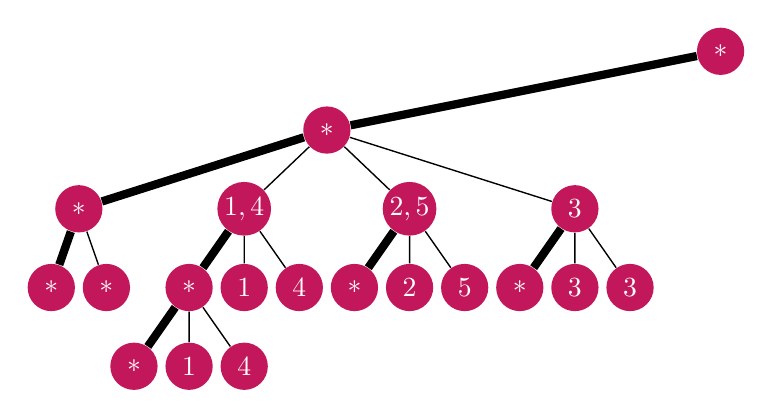
\begin{tikzpicture}[
  level distance=10mm,
  every node/.style={circle,white,minimum size=6mm,inner sep=1pt, fill=pink, thin},
  level 1/.style={sibling distance=50mm},
  level 2/.style={sibling distance=21mm},
  level 3/.style={sibling distance=7mm},
]
\node {$*$}
  child [pv] {node {$*$}
    child [pv] {node {$*$}
      child [pv] {node {$*$}}
      child [nonpv] {node {$*$}}
    }
    child [nonpv] {node {$1,4$}
      child [pv] {node {$*$}
        child [pv] {node {$*$}}
        child [nonpv] {node {$1$}}
        child [nonpv] {node {$4$}}
      }
      child [nonpv] {node {$1$}}
      child [nonpv] {node {$4$}}
    }
    child [nonpv] {node {$2,5$}
      child [pv] {node {$*$}}
      child [nonpv] {node {$2$}}
      child [nonpv] {node {$5$}}
    }
    child [nonpv] {node {$3$}
      child [pv] {node {$*$}}
      child [nonpv] {node {$3$}}
      child [nonpv] {node {$3$}}
    }
  }
  child[missing]
  child[missing];
\end{tikzpicture}
\end{document}